\begin{enumerate}[\Large\bfseries 1.]

%--------------------1.
\item \textbf{\large COMPOSICIÓN DE FUNCIONES}\\\\

    \begin{enumerate}[\bfseries a)]

	%----------a.
	\item \textbf{(George Thomas, Calculo una variable, capítulo 1)}\\\\ 
	    Escribir una fórmula para $f\circ g \circ h$.  $f(x)=\sqrt{x+1},\quad \dfrac{1}{x+4}, \quad h(x)=\dfrac{1}{x}$\\\\ 
	    Respuesta.-\; $f(g(h(x))) = f\left(g \left(\dfrac{1}{x}\right) \right) = f\left(\dfrac{1}{\dfrac{1}{x} + 4}\right) = \sqrt{\dfrac{1}{\dfrac{1}{x} + 4} + 1} = \sqrt{\dfrac{5x+1}{4x+1}}$ para $ x \neq 0, -\dfrac{1}{4}$.\\\\

	%----------b)
	\item \textbf{Código fuente.}\\ 
	    
	    \lstinputlisting[language=Python]{python/tareas_mat/week4/compo1.py}
	    \vspace{.5cm}
	
	%----------c)
	\item \textbf{Prueba de la ejecución del programa}.\\
	    \begin{center}
		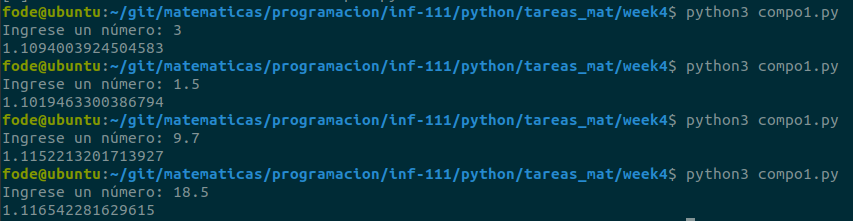
\includegraphics[scale=.5]{imagenes/tareas_mat/week4/compo1.png}
	    \end{center}

    \end{enumerate}

\newpage

%--------------------2.
\item \textbf{\large COMPOSICIÓN DE FUNCIONES}\\\\

    \begin{enumerate}[\bfseries a)]

	%----------a.
	\item \textbf{(George Thomas, Calculo una variable, capítulo 1)}\\\\ 
	Escribir una fórmula para $f\circ g \circ h$. $f(x)=\dfrac{x+2}{3-x}, \quad g(x)=\dfrac{x^2}{x^2+1}, \quad h(x)=\sqrt{2-x}$\\\\
	    Respuesta.-\; $f\left( g \left( \sqrt{2-x}\right)\right) = f\left( \dfrac{|2-x|}{|2-x|+1}\right) = \dfrac{\dfrac{|2-x|}{|2-x|+1} + 2}{3 - \left(\dfrac{|2-x|}{|2-x|+1}\right)}$\\\\

	%----------b)
	\item \textbf{Código fuente.}\\ 
	    
	    \lstinputlisting[language=Python]{python/tareas_mat/week4/compo2.py}
	    \vspace{.5cm}
	
	%----------c)
	\item \textbf{Prueba de la ejecución del programa}.\\
	    \begin{center}
		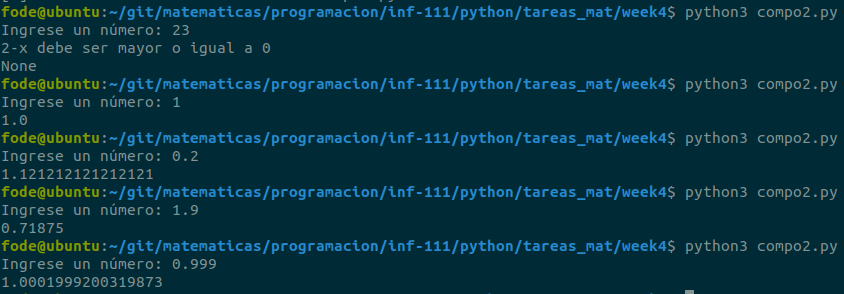
\includegraphics[scale=.5]{imagenes/tareas_mat/week4/compo2.png}
	    \end{center}

    \end{enumerate}

\newpage

%--------------------3.
\item \textbf{\large DESPLAZAMIENTO DE FUNCIONES}\\\\

    \begin{enumerate}[\bfseries a)]

	%----------a.
	\item \textbf{(George Thomas, Calculo una variable, capítulo 1)}\\\\ 
	La siguiente figura muestra la gráfica de $y = -x^2$ desplazada a dos posiciones nuevas. Escriba las ecuaciones de las gráficas nuevas.\\\\
	    Respuesta.-\; 
	    \begin{enumerate}[a)]
		\item $y=-(x+7)^2$\\
		\item $y=-(x-4)^2$\\\\
	    \end{enumerate}


	%----------b)
	\item \textbf{Código fuente.}\\ 
	    
	    \lstinputlisting[language=Python]{python/tareas_mat/week4/grafica1.py}
	    \vspace{.5cm}
	
	%----------c)
	\item \textbf{Prueba de la ejecución del programa}.\\
	    \begin{center}
		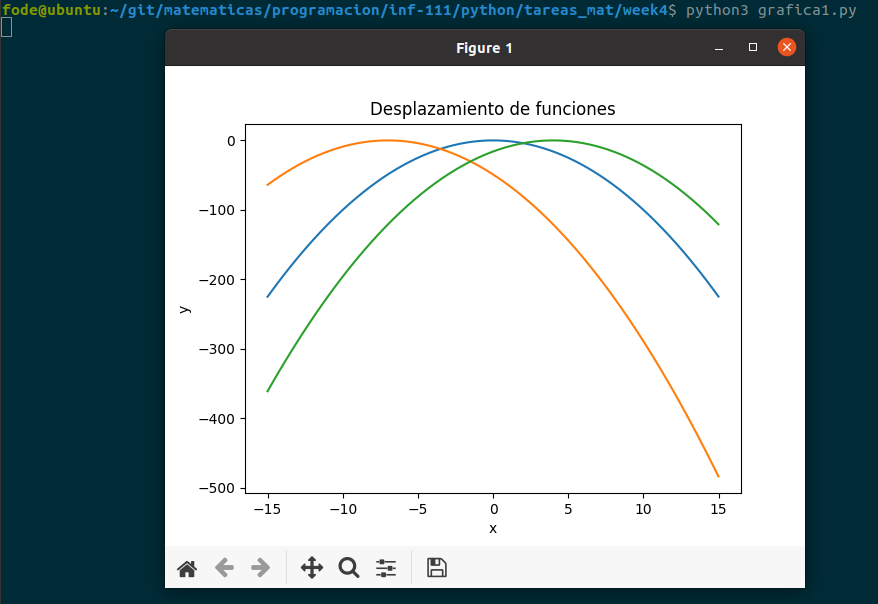
\includegraphics[scale=.4]{imagenes/tareas_mat/week4/grafica1.png}
	    \end{center}

    \end{enumerate}

\newpage

%--------------------4.
\item \textbf{\large DESPLAZAMIENTO DE FUNCIONES}\\\\

    \begin{enumerate}[\bfseries a)]

	%----------a.
	\item \textbf{(George Thomas, Calculo una variable, capítulo 1)}\\\\ 
	    La siguiente figura muestra la gráfica de $y=x^2$ desplazada a dos posiciones nuevas. Escriba las ecuaciones de las gráficas nuevas.\\\\
	    Respuesta.-\; 
	    \begin{enumerate}[a)]
		\item $y=x^2 + 3$\\
		\item $x^2 - 5$\\\\
	    \end{enumerate}

	%----------b)
	\item \textbf{Código fuente.}\\ 
	    
	    \lstinputlisting[language=Python]{python/tareas_mat/week4/grafica2.py}
	    \vspace{.5cm}
	
	%----------c)
	\item \textbf{Prueba de la ejecución del programa}.\\
	    \begin{center}
		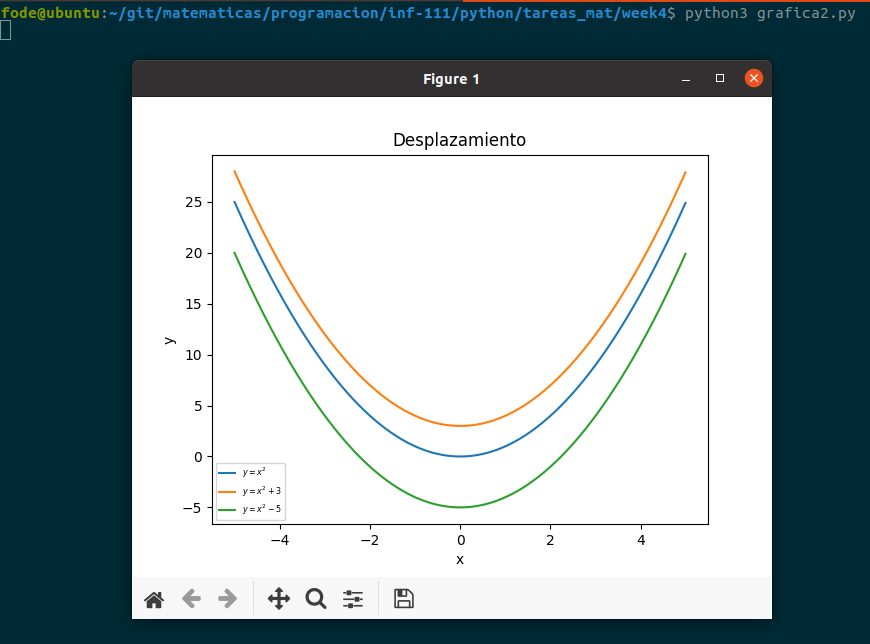
\includegraphics[scale=.4]{imagenes/tareas_mat/week4/grafica2.png}
	    \end{center}

    \end{enumerate}

\newpage

%--------------------5.
\item \textbf{\large DESPLAZAMIENTO DE FUNCIONES}\\\\

    \begin{enumerate}[\bfseries a)]

	%----------a.
	\item \textbf{(George Thomas, Calculo una variable, capítulo 1)}\\\\ 
	    Relacione las ecuaciones listadas en los incisos $a)$ a $d)$ con las gráficas de la figura.\\\\
		Respuesta.-\;
		\begin{enumerate}[\bfseries a)]

		    %----------a)
		    \item $y=(x-1)^2 - 4 = $ Posición 4.\\

		    %----------b)
		    \item $y=(x-2)^2 + 2 = $ Posición 1.\\

		    %----------c)
		    \item $y=(x+2)^2 + 2 = $ Posición 2.\\

		    %----------d)
		    \item $y=(x+3)^2 - 2 = $ Posición 3.\\\\
		\end{enumerate}

	%----------b)
	\item \textbf{Código fuente.}\\ 
	    
	    \lstinputlisting[language=Python]{python/tareas_mat/week4/grafica3.py}
	    \vspace{.5cm}
	
	%----------c)
	\item \textbf{Prueba de la ejecución del programa}.\\
	    \begin{center}
		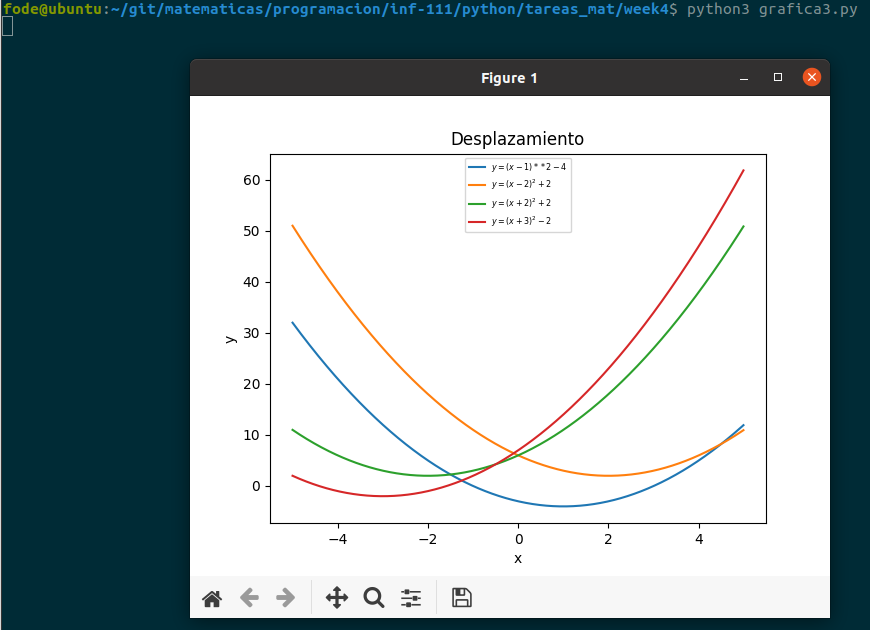
\includegraphics[scale=.35]{imagenes/tareas_mat/week4/grafica3.png}
	    \end{center}

    \end{enumerate}

\newpage
\end{enumerate}
